\section {Case Studies}

This section presents some initial results of applying normalization
and generalization.   All tests were generated using
random testing.  We also tested the Python interface to Z3 \cite{z3},
but did not find faults thus far, though normalization did help produce more
comprehensible and uniform
quick tests \cite{icst2014}.

\subsection{AVLTree}

For basic experiments on the ability of normalization to reduce the
number of failing test cases and preserve fault detection, we used a
simple Python implementation of AVL trees found on the web
\cite{avltree}, with 225 lines of code\footnote{All code sizes non-comment, non-blank lines, measured by cloc \cite{cloc}.}.

\begin{figure}
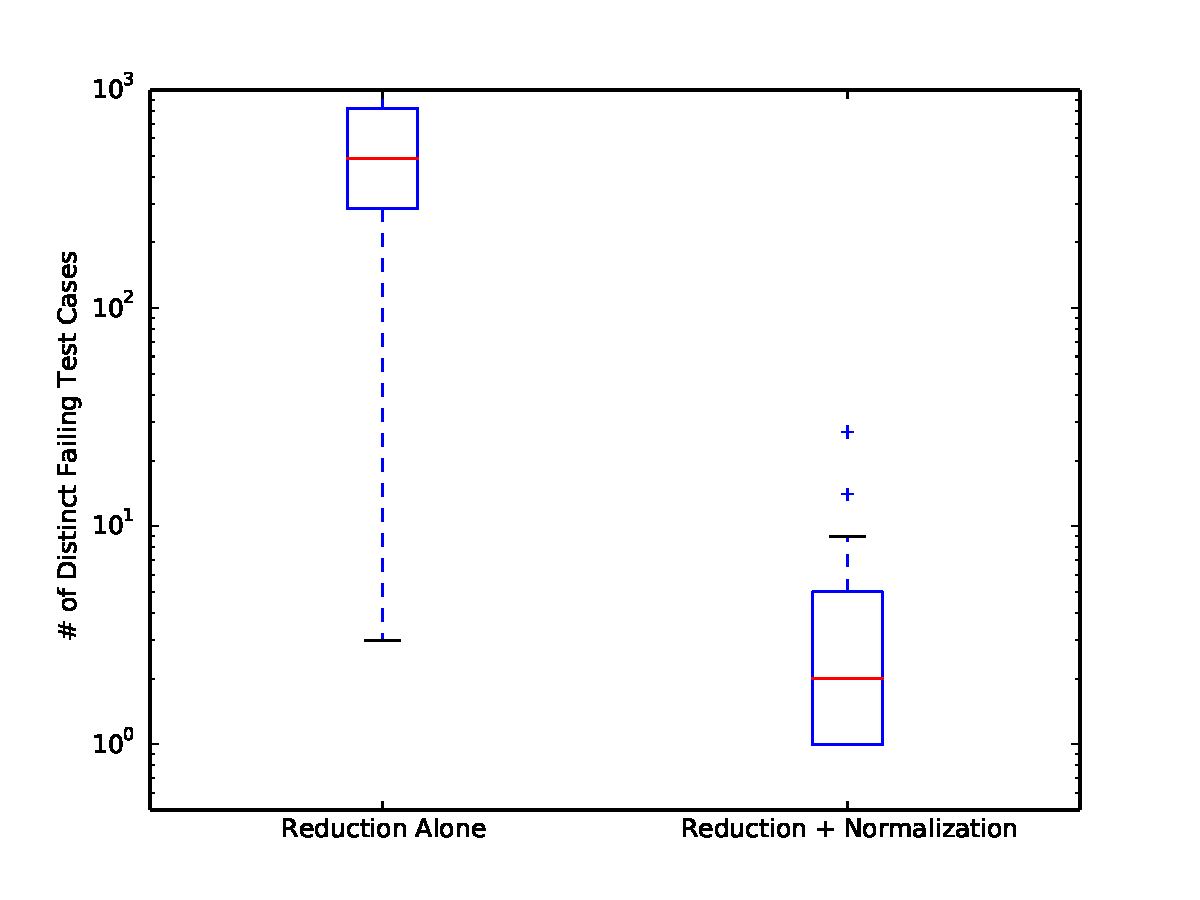
\includegraphics[width=\columnwidth]{length}
\caption{Effects of normalization on 82 AVL Tree mutants.}
\label{normeffect}
\end{figure}

Figure \ref{normeffect} shows the reduction in number of distinct
failing test cases produced by normalization (vs. reduction only) for
a set of 82 mutants \cite{mutant} of the AVLTree source code \cite{Hunter:2007}.  Of the 228 mutants
produced by MutPy \cite{mutpy}, only these produced at least 1 failure
in 1,000 test cases.  Using only delta-debugging-based reduction, the
mean number of distinct failures for each mutant (which is, by definition,
a single fault) was 498.4, with a median of 485.  Using normalization,
the mean was 3.1 distinct failures, with a median of just 2 failures.
For 38 of the 82 mutants, normalization produced only a single
representative failure.  For every mutant, normalization reduced the
number of distinct failures, and no mutant produced more than 27
distinct failures, after normalization.

The mean cost to reduce a
test case was 0.05 seconds, with a median of 0.03 seconds.  The mean
cost for normalization was 0.38 seconds, with a median of 0.1 seconds.
The minimum runtime for both algorithms was negligible (less than 1
millisecond), but the maximums were 1.3 seconds for reduction and 17.6
seconds for normalization.  Note that in all our results the cost of
normalization is given on an already-reduced test case, so the inputs
for normalization are smaller than those for reduction; however, this
is the expected use-case for normalization.  Comparing on equal-sized
tests would simply involve adding the costs for reduction to those for
normalization, as an additional step of normalization.  Finally, the
criticality of caching for normalizing large numbers of tests is
evident.  Out of 60,226 normalizations performed in our full AVLTree mutant
experiments, 59,972 (99.6\%) resulted in a cache hit (most of these
after a small number of normalization steps).  In fact, the total
number of rewrites performed during the experiments was only 145,780,
for an average of only 2.4 non-cache-hit rewrites of each test.  Note
that this is with the cache starting empty for each of the 82 mutants.

AVLTree mutants also provided a way to evaluate the danger of
normalization losing faults by changing a test case failing due to one
fault into a test case failing due to a different fault, a problem
known as ``slippage'' when it occurs with delta-debugging
\cite{PLDI13}.  AVLTree is a particularly challenging setting in this
regard, as there are very few API calls, and all calls take the same
simple inputs, so test cases for faults are likely to be very close to
each other in the combinatorial space.  To test the slippage rates for
normalization, we randomly selected 364 mutant pairs drawn from the 82
detectable mutants, and produced higher-order-mutants for each of
these by applying both mutants (using only mutants that modified
different source lines).  Of these, the set of reduced test cases
included at least one test capable of exposing each of the two faults
for only 238 pairs (in almost all cases due to reduction slippage, but
in a few cases due to one fault completely masking the other fault:  e.g., if
{\tt insert} always fails, it is not possible to produce a test case
that exposes a fault in {\tt delete} on a non-empty tree).

Out of these 238 mutant pairs, normalization produced test cases
exposing both faults for 80.7\% of pairs (19.3\% slippage at the
suite level).  Interestingly, in 4 cases
normalization took a set of reduced test cases not capable of exposing
both faults, and produced a smaller set of test cases that was capable
of detecting both faults (this is not counted into the slippage
measure).  Arguably this is ``slippage'' in that a test case not
capable of exposing fault F was modified to expose fault F (classic
slippage) but since the new test suite exposed both faults,
normalization actually restored fault detection.

Data on slippage is not extensive (in part because few actual testers
read unreduced test cases, so it is only detected if the original test
cases before reduction are stored and re-executed after bugs have been
fixed), but in our own previous work \cite{PLDI13}, slippage due to
reduction was extremely rare for some SUTs (GCC 4.3.0) and very common
for other SUTs (up to 23\% for Mozilla's JavaScript engine).  For our
own AVLTree example, the slippage rate for reduction (ignoring
normalization) is almost 30\%.  As a simple mitigation, we propose
storing at least reduced test cases, and ideally the original,
unreduced test cases, as a
slippage check when all faults detected by normalized test cases
are fixed.  

The reduction in test cases produced by normalization for mutant pairs
was, as with single mutants, very large (Figure \ref{normeffect}).
For mutant pairs, the mean/median number of distinct failures was
554.4/607 for reduction alone, but only 2.8/2 for reduction +
normalization.  The runtime for normalization was essentially
unchanged from the single-mutant numbers given above.  For reduction
alone, using pairs increased the number of distinct failures, while
normalized failure counts actually decreased.  For 48.3\% (115 of 238) of
mutant pairs where reduction did not lose a fault, normalization was
``perfect'' --- it preserved both faults and produced only 1 or 2 test
cases\footnote{It is possible to detect both faults with a single test
  case, if that test case fails when \emph{either} fault is
  present.}. 

\subsection{XML Parser}

We also examined how normalization combined with multiple faults for a
simple XML parser with about 260 lines of code \cite{myxml}, with one
real fault, triggered by the empty tag ({\tt <>})), and one
seeded fault triggered when adding two nodes with the same
name.  A comment in the code indicates the seeded fault is realistic.  Running 1,000 tests
produced 848 failing test cases.  Without normalization, it took only
37.45 seconds to execute and delta-debug all 1,000 tests.  The output was 717 distinct failing test
cases.  Normalization increased the runtime to 354.7 seconds, but
reduced the number of failures to just 5: 3 failures
for the original fault and 2 for the seeded fault.
%Generalization took < 5 seconds.


\subsection{TSTL}

As noted in Section \ref{freshgen}, TSTL is used to test TSTL's own API
interface (the TSTL compiler is about 1,600 LOC; a compiled SUT is
often 30KLOC or larger).  For the only fault discovered so far in
testing the latest version of TSTL, the cache-related problem mentioned above, generating
and reducing 100 test cases required 1,090 seconds and produced 90 failures.  Adding normalization and generalization increased
the runtime to 3,690 seconds, but produced just two failures.

\subsection{NumPy}

Our final two case studies provide little information on the ability
of normalization to reduce the number of failing tests; for these
SUTs, failure rates are low enough or test case reduction runtimes high
enough that each failure is dealt with one-by-one.  However,
normalization and generalization are, we claim, also useful for
individual test cases.

NumPy \cite{NumPy} is a very widely used Python library/extension that
supports large, multi-dimensional matrices and provides a huge library
of mathematical functions.  The popular SciPy library for scientific
computing builds on NumPy.  Developing tests for NumPy is challenging,
because none of the authors are experts in numeric computation, and
the specification of correct behavior is often somewhat subtle.  As a
simple example, consider the test case in Figure \ref{numpyorig},
normalized and generalized in Figure \ref{numpynormgen}.  Prior to
normalization, understanding why the test case leads to a violation of
self-equality for an array is, to say the least, non-trivial.  After
normalization, it is much clearer what is happening: 1) {\tt array0}
contains {\tt NaN} 2) this is in fact correct behavior (the array
\emph{should} contain {\tt NaN}).  The greater length and much larger
number of operations involved in the original reduced test case
obscures this critical point.  In NumPy, array equality does not hold
for objects containing {\tt NaN}, so the assertion must be modified.
As far as we know, normalization transforms all instances of this
fault into this canonical test case, but our data (over fewer than 30
failures) is insufficient to make a definite claim, as the failure rate
is slightly less than 3 failures/100,000 tests on average.


Other, more complex, failures have also made it clear that normalization
is useful for additional test case length reduction for NumPy, and
that generalization makes any surprising restrictions on test values
clear.  For NumPy tests, normalization takes much longer than
reduction, in part due to the expense of operations on large arrays.
Over almost all examples, the average time to reduce tests is about
4-5 seconds, and the time for normalization is between 712 and 774
seconds.  The average time to discover a failing test case, for
comparison, is just over 400 seconds.  Generalization takes between 52
and 59 seconds in these cases.  The exception was a test case of
45,206 steps (!)  leading to a memory exhaustion error and crash,
reduced (over a period of nearly a day) to a test case with 10 steps,
which then normalized (in only 2 hours) to a test case with 8 steps,
involving no operations other than array initialization (with zeros or
ones), array flattening, and array addition (the original test case
involved larger dimensions, array multiplication, and array
subtraction).  This is the only case in which we have seen
normalization time lower than reduction time, without assistance from
the cache.

\begin{figure}
{\scriptsize
\begin{code}
 dim1 = 1 
 shape2 = (dim1, dim1, dim1) 
 array1 = np.ones(shape2) 
 array0 = array1 * array1 
 array1 = array1 + array1 
 array4 = array0 + array1 
 array0 = np.reshape(array4,shape2) 
 array3 = array1 * array4 
 array2 = np.ravel(array4) 
 array5 = array2 - array3 
 array4 = array5 * array2 
 array1 = np.unique(array0) 
 array5 = array5 * array3 
 array0 = array1 * array5 
 array5 = np.unique(array0) 
 array1 = array4 - array2 
 array2 = array0.flatten() 
 array0 = array5 + array5 
 array5 = array5 + array2 
 array2 = array0 * array2 
 np.copyto(array5,array2) 
 array2 = array2 * array5 
 array3 = array0 * array2 
 array0 = array3 - array1 
 array4 = array3 * array0 
 array1 = array5 + array4 
 array5 = array0 * array1 
 array0 = array5 - array1 
 array4 = array0 * array3 
 array3 = array4 * array0 
 array1 = array5 + array3 
 array0 = array2 + array1 
 array5 = array5 - array0 
 array5 = array3 * array5 
 array0 = array1 + array5 
 array2 = array3 - array0 
 array4 = array2 * array1 
 array3 = array4 * array2 
 array2 = array0 - array0 
 np.copyto(array1,array3) 
 array4 = array2.flatten() 
 array1 = array1 * array4
 assert (np.array\_equal(array1,array1))
\end{code}
}
\caption{Original ``failing'' test case for numpy (42 steps).}
\label{numpyorig}
\end{figure}

\begin{figure}
{\scriptsize
\begin{code}
dim0 = 1                            \textcolor{black!60}{\# STEP 0}
\textcolor{black!60}{\#  or dim0 = 10 }
shape0 = (dim0)                     \textcolor{black!60}{\# STEP 1}
\textcolor{black!60}{\#  or shape0 = (dim0, dim0) }
\textcolor{black!60}{\#  or shape0 = (dim0, dim0, dim0) }
array0 = np.ones(shape0)            \textcolor{black!60}{\# STEP 2}
array0 = array0 + array0            \textcolor{black!60}{\# STEP 3}
array0 = array0 + array0            \textcolor{black!60}{\# STEP 4}
\textcolor{black!60}{\#  or array0 = array0 * array0 }
array0 = array0 * array0            \textcolor{black!60}{\# STEP 5}
array0 = array0 * array0            \textcolor{black!60}{\# STEP 6}
array0 = array0 * array0            \textcolor{black!60}{\# STEP 7}
array0 = array0 * array0            \textcolor{black!60}{\# STEP 8}
array0 = array0 * array0            \textcolor{black!60}{\# STEP 9}
array0 = array0 * array0            \textcolor{black!60}{\# STEP 10}
array0 = array0 * array0            \textcolor{black!60}{\# STEP 11}
array0 = array0 * array0            \textcolor{black!60}{\# STEP 12}
array0 = array0 * array0            \textcolor{black!60}{\# STEP 13}
array0 = array0 - array0            \textcolor{black!60}{\# STEP 14}
assert (np.array\_equal(array0,array0))
\end{code}
}
\caption{Normalized and generalized test case for numpy (15 steps).}
\label{numpynormgen}
\end{figure}

\subsection{Esri ArcPy}

Esri is the single
largest Geographic Information System (GIS) software vendor, with about 40\%
of global market share.  Esri's ArcGIS tools are extremely widely
used for GIS analysis, in government, scientific research, commercial
enterprises, and education.  Automation for complex GIS analysis and
data management is a frequent need, and Esri has long provided tools
for programming their GIS software systems.  The current method of
choice is a Python site-package, ArcPy \cite{ArcPy}.  ArcPy is a complex library,
with dozens of classes and hundreds of functions distributed over
a variety of of toolboxes.  Most of the code involved in ArcPy
functionality is C++ for which source is unavailable (the source for
the actual ArcGIS tools); the Python source alone is over 50,000 lines
of code.

In order to improve the reliability of ArcPy, we have been
implementing a TSTL-based framework for testing ArcPy itself as well
as libraries based on ArcPy.  The TSTL definition is already more than
twice as large as the next-largest example previously studied, even
though it only includes a small portion of ArcGIS so far. The first
stage of testing has resulted in discovery of multiple faults in
ArcPy/ArcGIS, six of which not only cause incorrect behavior but
cause a crash that also ends testing.  Before proceeding to more
nuanced testing, it is critical to understand these faults, the set of
behaviors that trigger them, and modify the test definition to avoid
triggering these faults with minimal limitations on thorough testing.

There is no space in this paper to elaborate on the details of this
large test effort (which has required adding numerous additional
features and modes to TSTL), but normalization and generalization have
been very useful in this process.  Figures \ref{esriorig} and
\ref{esrinormgen} show one crash-inducing test case, after initial
delta-debugging (from over 2,000 test steps) (Figure \ref{esriorig})
and with normalization and generalization (Figure \ref{esrinormgen}).
First, in this setting normalization has contributed a surprising
amount of additional reduction over delta-debugging.  In this example,
normalization reduced the length from 19 steps to 11 steps; in another
case, it reduced the test case from 18 to 14 steps, and in yet another
crash fault, it reduced the test case from 27 to 20 steps (one crash
fault only reduced from 10 steps to 9 steps, but the omission was
informative).  The cost of normalization is high --- in our runs, it
has taken from 17,340 seconds up to 24,769 seconds.  However, in this
setting even delta-debugging is extremely expensive --- the cost of
reduction alone has ranged from 7,930 seconds to 8,688 seconds.
Generalization has taken from under an hour (3,203 seconds) up to
11,149 seconds.  These costs are due in part to the need to run tests
in a sandbox environment to avoid killing the Python testing process,
and in part due to the cost of running complex GIS analyses.  However,
even with this high cost, reducing, normalizing, and generalizing test
cases has been a more effective use of our time than trying to
understand the faults without these aids.  For example, in the test
case shown in this paper, it was important to understand that the SQL
query and selection type were not essential, but using a freshly
created layer will not result in a crash: the problem appears to be
that ArcGIS (or ArcPy) does not invalidate layers built from a feature
class when that feature class is deleted\footnote{In this instance, a
  generalization (the fresh values generalization in particular) is
  informative even though it does not allow any generalization;
  knowing that it was attempted, but prevented the failure, is also
  valuable.}.  The original, non-normalized test case makes this far
less clear, as the use of {\tt CopyFeatures} and the multiplicity of
shapefiles involved disguises the essence of the problem.

In addition to helping us understand failures, normalization and
generalization are also being used to prepare an API-behavior
regression suite for ArcPy.  One of the challenges of using a large
API like ArcPy is that behavior of the system can change from version
to version; in some cases this is due to new faults, or fixed faults,
but in other cases there is simply an undocumented change.  In order
to assist ArcPy developers, we are preparing a test suite that covers
as much as possible of the Python source for ArcPy, in the latest version of ArcPy,
10.3, and records the values returned in 10.3.  For future versions of
ArcPy (or older versions), a ``semantic diff'' with 10.3, based on
these calls, can be produced by running this suite.  The tests in the
suite are normalized and generalized to help users understand the
conditions behind an API usage's behavior, not just one set of
values.  This ``coverage regression'' quick test \cite{icst2014} may
also be useful for helping users understand the API, since the set of
online examples of usage from Esri is usually limited to a small set
of parameter combinations.

\begin{figure}
{\scriptsize 
\begin{code}
shapefile2 = "C:\\arctmp\\new3.shp" 
shapefile1 = "C:\\arctmp\\new3.shp" 
featureclass2 = shapefile2 
featureclass0 = shapefile1 
shapefilelist2 = 
   glob.glob("C:\\Arctmp\\*.shp") 
fieldname0 = "newf3" 
shapefile1 = shapefilelist2 [0] 
featureclass1 = shapefile1 
arcpy.CopyFeatures\_management
   (featureclass1,featureclass2) 
op1 = ">" 
newlayer2 = "l2" 
val1 = "100" 
selectiontype2 = "SWITCH\_SELECTION" 
fieldname1 = "newf1" 
arcpy.MakeFeatureLayer\_management
   (featureclass0, newlayer2) 
arcpy.SelectLayerByAttribute\_management
   (newlayer2,selectiontype2,
   ' "'+fieldname0+'" '+op1+val1) 
op0 = ">" 
arcpy.Delete\_management(featureclass2) 
arcpy.SelectLayerByAttribute\_management
   (newlayer2,selectiontype2,
   ' "'+fieldname1+'" '+op0+val1) 
\end{code}
}
\caption{Original test case for ArcPy library (19 steps).}
\label{esriorig}
\end{figure}

\begin{figure}
{\scriptsize 
\begin{code}
shapefilelist0 = 
   glob.glob("C:\\Arctmp\\*.shp")        \textcolor{black!60}{\# STEP 0}
\textcolor{black!60}{\#[}
shapefile0 = shapefilelist0 [0]        \textcolor{black!60}{\# STEP 1}
newlayer0 = "l1"                       \textcolor{black!60}{\# STEP 2}
\textcolor{black!60}{\#  or newlayer0 = "l2" }
\textcolor{black!60}{\#  or newlayer0 = "l3" }
\textcolor{black!60}{\#  swaps with steps 3 4 5 6 7}
\textcolor{black!60}{\#] (steps in [] can be in any order)}
\textcolor{black!60}{\#[}
featureclass0 = shapefile0             \textcolor{black!60}{\# STEP 3}
\textcolor{black!60}{\#  swaps with step 2}
fieldname0 = "newf1"                   \textcolor{black!60}{\# STEP 4}
\textcolor{black!60}{\#  or fieldname0 = "newf2" }
\textcolor{black!60}{\#  or fieldname0 = "newf3" }
\textcolor{black!60}{\#  swaps with steps 2 8}
selectiontype0 = "SWITCH\_SELECTION"    \textcolor{black!60}{\# STEP 5}
\textcolor{black!60}{\#  or selectiontype0 = "NEW\_SELECTION" }
\textcolor{black!60}{\#  or selectiontype0 = "ADD\_TO\_SELECTION" }
\textcolor{black!60}{\#  or selectiontype0 = "REMOVE\_FROM\_SELECTION"}
\textcolor{black!60}{\#  or selectiontype0 = "SUBSET\_SELECTION"}
\textcolor{black!60}{\#  or selectiontype0 = "CLEAR\_SELECTION"   }
\textcolor{black!60}{\#  swaps with steps 2 8}
op0 = ">"                              \textcolor{black!60}{\# STEP 6}
\textcolor{black!60}{\#  or op0 = "<" }
\textcolor{black!60}{\#  swaps with steps 2 8}
val0 = "100"                           \textcolor{black!60}{\# STEP 7}
\textcolor{black!60}{\#  or val0 = "1000" }
\textcolor{black!60}{\#  swaps with steps 2 8}
\textcolor{black!60}{\#] (steps in [] can be in any order)}
arcpy.MakeFeatureLayer\_management
   (featureclass0, newlayer0)          \textcolor{black!60}{\# STEP 8}
\textcolor{black!60}{\#  swaps with steps 4 5 6 7}
arcpy.SelectLayerByAttribute\_management
   (newlayer0,selectiontype0,
   ' "'+fieldname0+'" '+op0+val0)      \textcolor{black!60}{\# STEP 9}
arcpy.Delete\_management(featureclass0) \textcolor{black!60}{\# STEP 10}
arcpy.SelectLayerByAttribute\_management
   (newlayer0,selectiontype0,
   ' "'+ fieldname0+'" '+op0+val0)     \textcolor{black!60}{\# STEP 11}
\end{code}
}
\caption{Normalized and generalized test case for ArcPy library
  (12 steps).}
\label{esrinormgen}
\end{figure}